\ssection{Results}
\label{sec:results}

BREW-RC cannot infer the number of parity bits ($r$), therefore we run for $r \in \{1,..,k\}$, corresponding to all candidate matrices up to a code rate of 0.5. BREW-RC returns a single parity submatrix satisfying a single $r$ for both the 4M and 8M. 

Parity matrices are considered sensitive trade secrets. As in \cite{patel2020bit}, we do not provide the exact parity matrices here. Instead, we use our extracted parity submatrix to predict timing measurements for a fresh validation set of 1-word random unipolar walk test vectors.  

\ssubsection{Timing Model Construction}

Two systematic generator matrices ($G_{4M}$ and $G_{8M}$) are constructed by augmenting $I_{k_{4M}}$ and $I_{k_{8M}}$ with the extracted parity matrices $P_{4M}$ and $P_{8M}$, respectively. $G_{4M}$ and $G_{8M}$ are used to generate codeword transitions ($c_0$, $c_1$) corresponding to the dataword transitions  ($d_0$,$d_1$) produced by our prior unipolar random walk experiment. With full knowledge of the codeword transitions, it is now possible to compute the DHD for the codewords corresponding to each test vector. We separate 4M and 8M $t_w$ measurements from the prior random unipolar walk experiment and the median $t_w$ is computed for test vectors with identical $\left( w_{0\to1}, w_{1\to0} \right)$. The timing model for each device is defined as a lookup table with keys $\left( w_{0\to1}, w_{1\to0} \right)$ (DHD) returning an expected (median) write time ($\hat{t}_w$) for a given DHD ($\delta$) computed from a known codeword
{
\setlength{\abovedisplayskip}{2pt}
\setlength{\belowdisplayskip}{2pt}
\begin{equation}
    \hat{t}_w\left( \delta\right) = Med\left( t_w | DHD=\delta\right). 
\end{equation}
}
For comparison, this technique is repeated to generate a na\"ive timing model that uses datawords rather than codewords to generate DHDs and timing estimates. 
\ssubsection{Timing Model Performance}

\begin{figure}[t]
    \centering
    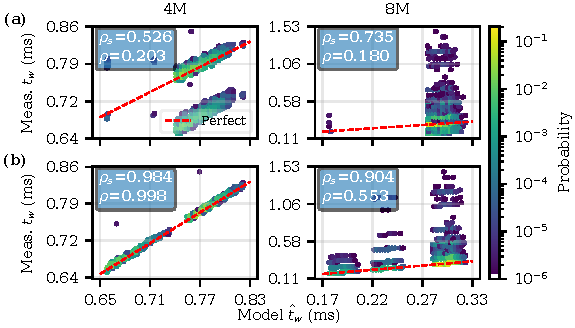
\includegraphics[width=\linewidth]{fig/images/pdf/model-comparison-codeword-vs-data.pdf}
    \vspace{-.75cm}
    \caption{Comparison of na\"ive dataword (a) and proposed codeword (b) timing models for 4M and 8M memories. Each point is colored according to the log probability that a measured $t_w$ occurs given a modeled $\hat{t}_w$.}
    % \vspace{-.2cm}
    \label{fig:timing-model}
\end{figure}

A fresh set of test vectors are generated for all 4M and 8M samples using Alg. \ref{alg:ruw}. For the na\"ive model ($d_0$,$d_1$) transitions from this test set are used directly to compute corresponding DHDs and lookup timing estimates. For our proposed model, $G_{4M}$ and $G_{8M}$ are used to produce codewords and the corresponding codeword DHDs are used to lookup timing estimates.

The test-vectors are then applied to each chip and the raw $t_{w}$ is captured (no aggregate statistics are taken). The ability of the proposed (BREW-RC-generated) timing model to predict the observed $t_{w}$ is compared to the na\"ive timing model in Figure \ref{fig:timing-model}. Both Spearman and Pearson correlation are shown as both are useful for side-channel analysis \cite{batina2008comparative}. On both chips the proposed timing model outperforms the na\"ive model. The proposed model explains almost all 4M $t_w$ variance, while rare long-tailed $t_w$ measurements present in the 8M limit improvements. These results demonstrate that the extracted parity submatrix yields a more accurate DHD, which improves timing leakage models.

% allowing for improved timing models that are critical to leakage modeling and security primitive design \cite{tolga2024trng, suri2018high}.

% Finally, we apply the test-vectors and generate $t_{wmin}$ cluster assignments ($\ell_{cw-meas}$) from the measured write latencies. We compare the ability of the BREW-RC-generated parity matrix to predict the observed $t_{ws}$ cluster with a na\"ive assignment from the data label $\ell_d$ in Figure \ref{fig:test-ruw}. The extracted parity matrices perfectly predict the cluster assignments for all applied validation $t_{ws}$ measurements. This result demonstrates that the parity matrix  